\documentclass{standalone}
\usepackage{tikz, tikz-cd}
\usetikzlibrary{shapes, decorations.markings, shapes.geometric}
\begin{document}
	
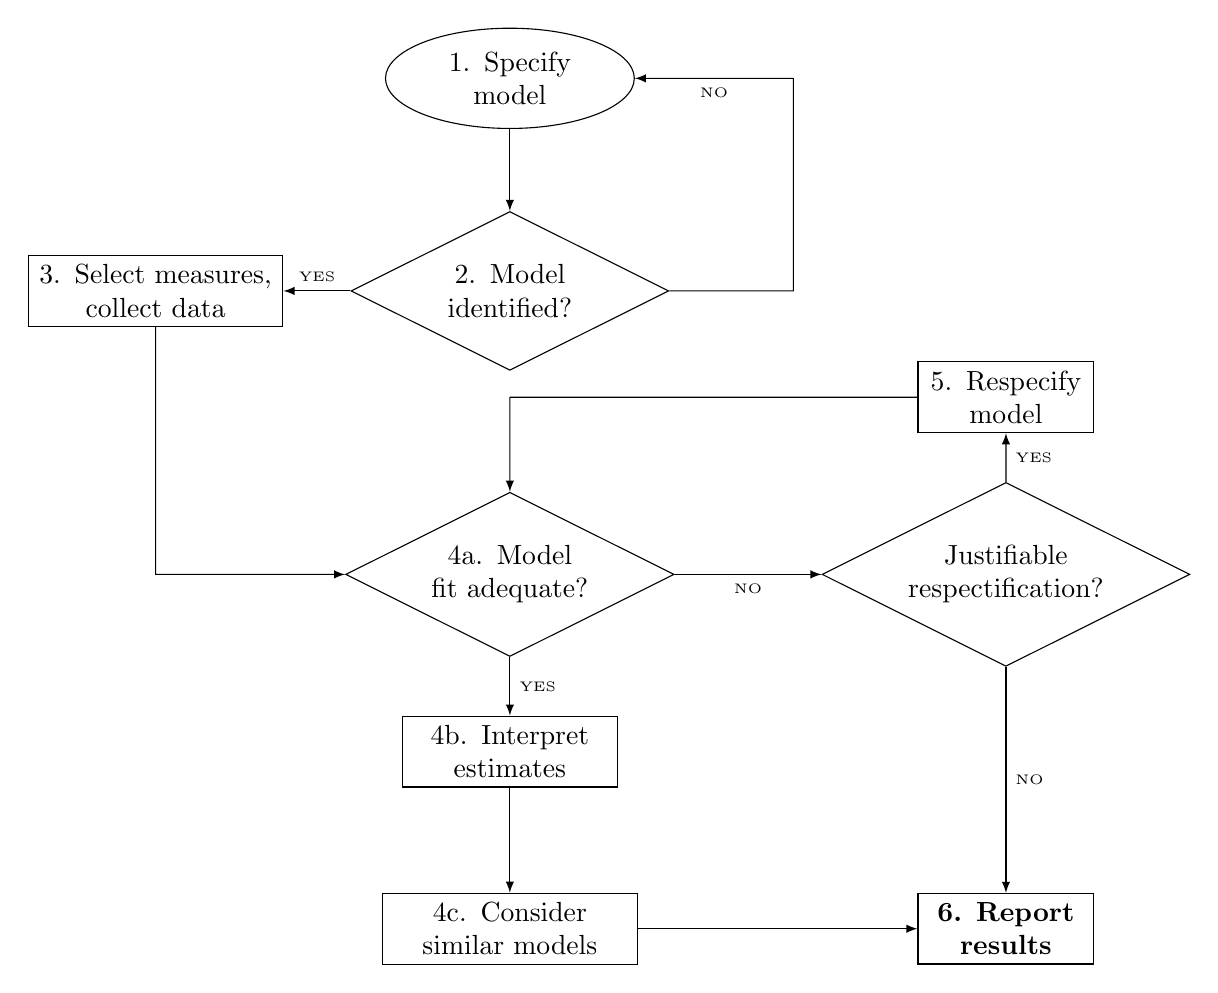
\begin{tikzpicture}[scale=0.9]
\node[draw, ellipse, text width=2cm, align=center] (s1) at (7,12) {1. Specify model};
\node[draw, diamond, text width=2cm, align=center, aspect=2] (s2) at (7,9) {2. Model identified?};
\node[draw, text width=3cm, align=center] (s3) at (2,9) {3. Select measures, collect data};
\node[draw, diamond, text width=2cm, align=center, aspect=2] (s4) at (7,5) {4a. Model fit adequate?};
\node[draw, text width=2.5cm, align=center] (s5) at (7,2.5) {4b. Interpret estimates};
\node[draw, text width=3cm, align=center] (s6) at (7,0) {4c. Consider similar models};
\node[draw, diamond, text width=2.5cm, align=center, aspect=2] (s7) at (14,5) {Justifiable respectification?};
\node[draw, text width=2cm, align=center] (s8) at (14,7.5) {5. Respecify model};
\node[draw, text width=2cm, align=center] (s9) at (14,0) {\textbf{6. Report results}};
% Arrows
\draw [->, thin, >=latex] (s1)--(s2.north);
\draw [->, thin, >=latex] (s2)--(s3.east) node [midway,above] {\tiny{YES}};
\draw [->, thin, >=latex] (s2.east) -| (11,12) -- node [midway, below] {\tiny{NO}} (s1.east);
\draw [->, thin, >=latex] (s3.south) -| (2,5) -- (s4.west);
\draw [->, thin, >=latex] (s4)--(s5.north) node [midway,right] {\tiny{YES}};
\draw [->, thin, >=latex] (s5)--(s6.north);
\draw [->, thin, >=latex] (s7)--(s8.south) node [midway,right] {\tiny{YES}};
\draw [->, thin, >=latex] (s8.west) -| (7,7.5) -- (s4.north);
\draw [->, thin, >=latex] (s4)--(s7.west) node [midway,below] {\tiny{NO}};
\draw [->, thin, >=latex] (s7)--(s9.north) node [midway,right] {\tiny{NO}};
\draw [->, thin, >=latex] (s6)--(s9.west);
\end{tikzpicture}
	
\end{document}